\documentclass[12pt,twoside,a4paper]{article}
\usepackage{titlesec}
\usepackage{chngcntr}
\usepackage{float}
\counterwithin{figure}{section}
\counterwithin{figure}{subsection}
\usepackage[margin=25mm]{geometry}
\linespread{1}
\titleformat*{\section}{\fontsize{14pt}{2}\bfseries}
\titleformat*{\subsection}{\fontsize{13pt}{2}\bfseries}
\titleformat*{\subsubsection}{\fontsize{13pt}{2}\bfseries}
\usepackage[T1]{fontenc}
\usepackage{mathptmx}
\usepackage{graphicx}
\usepackage{enumitem}
\graphicspath{ {imgs/} }

\begin{document}

\tableofcontents

The scope of this work is process of creating a device that automatically assigns broken eggs one of the three following classes: intact yolk, damaged yolk, clear line.
The implementation of such device will be preceded with research that compares various methods of recognizing the camera image, taking into account their performance in terms of computation resources, and in terms of correctness of the recognition

\section{Introduction}
\subsection{Research scope}
In 2014 creation of  camera based  module for chicken egg processing machines was requested by OVO-TECH company (the client).
The module is supposed to increase quality of egg-mass based  products made with use of  client machines.

During last 4 years multiple attempts were made by client to separate whites from yolks of freshly broken eggs in a mechanic way. 
Obtained solutions proved to be working good enough for some companies, while other rejected them as imperfect and declared will to buy clients devices in the future, provided that adequate improvements will be made.

The scope of this thesis is overviewing the possibilities of resolving client needs with image processing mechanisms that will optically detect state of object (batch of  intermediate product) and judge whether or not it should be discarded from the processing plant.
Moreover, a process of creating a prototype device using tested method  is described.

Problems such as:
- choosing image preprocessing methods
- finding optimal  parameters for used image alternations
- overfitting issues
- real-device solution implementation, 
- technical issues concerning the device choice, setup and performance 
had been taken  into account during the research procedure.






\begin{figure}[H]
\centering
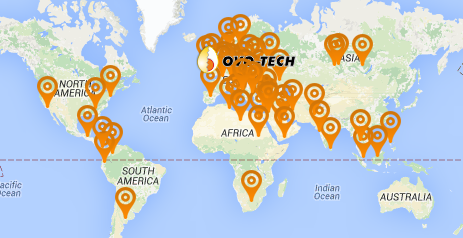
\includegraphics[width=0.4\paperwidth]{map}
\caption{Clients egg braking machines operating over the world}
\end{figure}

Figure 1.1 Clients egg braking machines operating over the world


\subsection{Host machine}
The machine that will be extended with the module prototype prepared in this thesis is OVO-TECH RZ-1 model.

\begin{figure}[H]
\centering
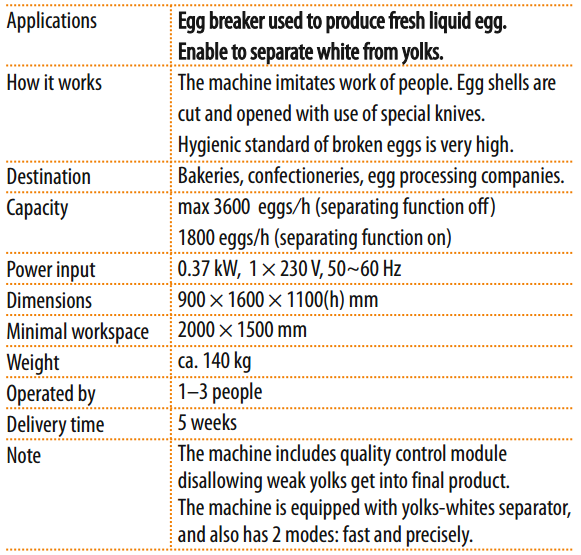
\includegraphics[width=0.4\paperwidth]{rz1table}
\caption{Rz-1 unit baisic parameters}
\end{figure}


\begin{figure}[H]
\centering
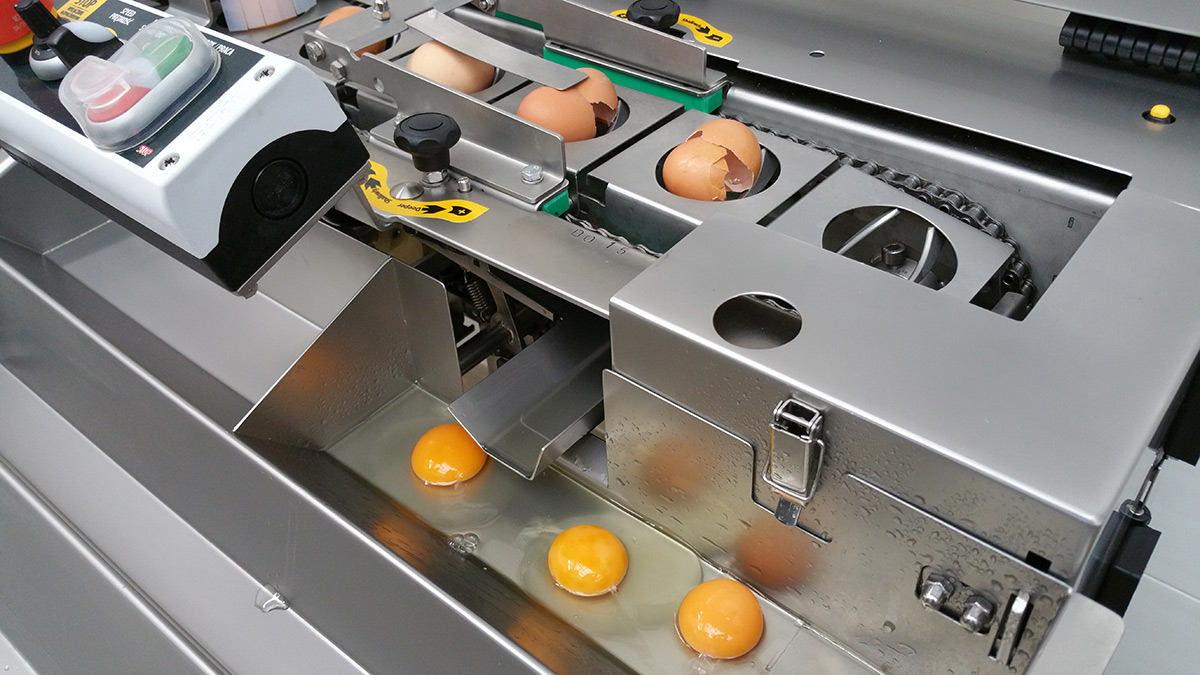
\includegraphics[width=0.4\paperwidth]{rz1crack}
\caption{Egg cracking  module of RZ-1 unit}
\end{figure}


The machine operates in a following way:
\begin{enumerate}
\item Eggs are directed into one-line flow, and mechanically aligned

\item Cracking module cuts the incoming egg surface from below with two knives that are aligned in direction of egg focal radius
\item The knives imitate human hands work by opening the previously notched egg
\item The cracked eggs are accumulated in a movable utensil for optical assessment. 
If the egg yolk appears to be broken, it is removed by an operator from the processing plant
\item Cracked eggs are transported by sliding to white and yolk separating module
\item Separation  is done in a mechanic way while eggs slide over specificly shaped gap that only egg white fills in, while the egg yolks remain intact
\end{enumerate}

\begin{figure}[H]
\centering
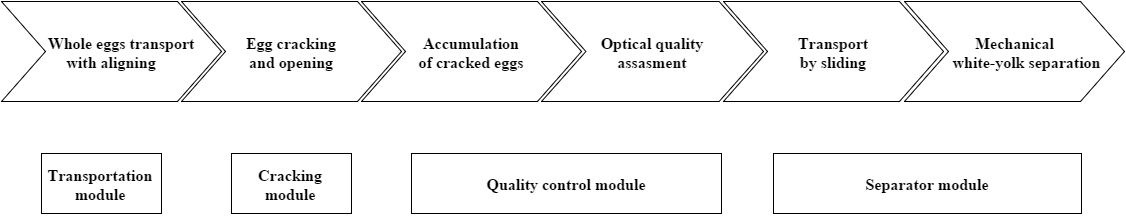
\includegraphics[width=0.8\paperwidth]{process}
\caption{RZ-1 Egg processing  - process and plant structure}

\end{figure}

RZ-1 operates in two modes:
- Precision mode
- Fast mode

Precision mode is used widely with bad quality eggs to extend amount of time for optical assessment in (5) phase.

More advanced OVO-TECH models such us RZ-3, RZ-6 and RZ-8 will be also considered for further research.

\subsection{Problem description}

If an egg processed by rz-1 machine is old or the chicken was feed improperly the yolk might be either broken already inside the egg, or might break during the cracking  phase due to cracker imperfections such us being calibrated for different size or weight eggs.
A mixture of damaged yolk and white is created in a result, and it’s not possible to separate it into two initial components using  the rz-1 separation  module.

Batch of such mixture should be removed from  the processing plant, since it would contaminate pure egg white product otherwise. 

\begin{figure}[H]
\centering
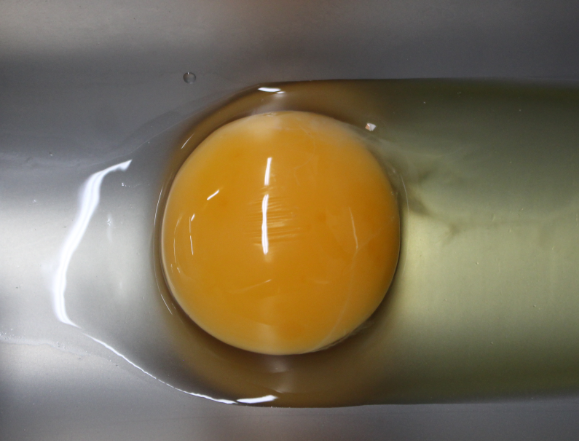
\includegraphics[width=0.4\paperwidth]{prop}
\caption{Properly cracked egg}
\end{figure} 

 
\begin{figure}[H]
\centering
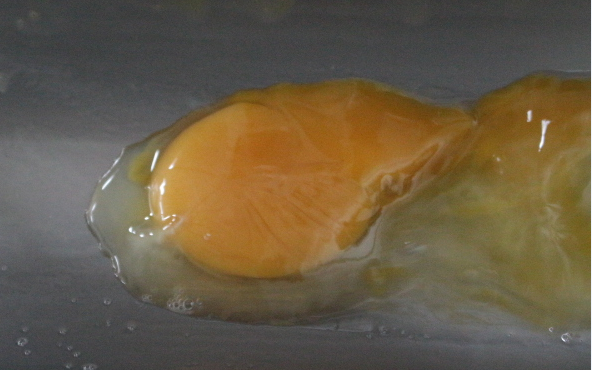
\includegraphics[width=0.4\paperwidth]{damg}
\caption{Damaged yolk in improperly cracked egg}
\end{figure}

\subsection{Demand for improvements}

Nine companies were inquired whether or not would they invest in improved Ovo-tech machine, provided that egg white will be visually clean of yolk parts. 
Seven of them replied positively that they would seriously consider such offer since their processing plants would benefit in terms of product quality or manpower cost on such improvement.
Remaining 2 companies did not answer the question.

One should consider why better separation is a requirement for those companies.
Following reasons were presented:

- Confectionaries and bakeries utilize egg white foam as an ingredient for their products. 
Egg white foam is obtained by aeration (also known as beating / foaming / whipping) process.
Comprehensive process description was provided by one of the bakers:

"When air is incorporated into a liquid or viscous solution, the solution entraps the air bubbles, forming a foam. If the foam is stabilized by proteins, it leavens a food, increasing its height and reducing its density. The viscosity of all egg products is ideal for incorporating air cells during the whipping or beating process. As whipping or beating progresses, air bubbles decrease in size and increase in number, all the time surrounded by egg proteins. Liquid egg products have low air-liquid interfacial tension; thus, when eggs are beaten or whipped, the proteins denature, or simply, they unfold. This exposes two oppositely charged ends of the protein molecule: the hydrophobic, or water-hating end, and the hydrophilic, or water-loving ends. The proteins align themselves between the air and water, securing the air bubbles with their hydrophilic chains pointing into the water and dangling their hydrophobic chains in the air. During baking, these proteins bond with each other, forming a delicate, yet reinforced network.

Egg whites do this much better than yolks because of the unique proteins found in whites. In fact, even though the term foam technically refers to any system where there are entrapped air bubbles, in the food industry, when discussing egg white products, the term tends to be exclusive to egg whites foams. This is because egg whites, unlike any other natural food ingredient, are able to create the largest possible food foam, a foam six to eight times greater in volume than unwhipped, non-aerated liquid egg white

Whole eggs and egg yolks can also increase the volume of foods, including certain baked goods and dairy desserts such as ice cream and custard, but just not as much as egg whites alone. Visually, whipped yolks may double or triple in volume, while whipped whole eggs produce less volume than either yolks or whites whipped separately. They are also less thick than yolks alone." \cite{eggprop}

- Ovo-tech observed that a simple dependence exists: the older the egg is, the more likely its yolk is degenerated inside the egg shell.
Thus eliminating the batches containing fuzzy yolk should decrease chances of accidentally processing the contaminated eggs, while the risk of egg contamination generally increases with egg age.

- One of the Ovo-tech clients is a biotechnology company that manufacture medicine out of genetically modified eggs.
The company purchased some ovo-tech machines, but is nevertheless displeased with their separation ratio.
This company currently is undergoing a procedure of obtaining US Food Drug Administration (FDA) approval for wide distribution of their egg-based medicine.
Executives of this client suspect that using machines with better egg separation will increase their chance for positive outcome of above process.
A non-disclosure agreement was signed between this client and ovo-tech, thus further expanding this topic in scope of this thesis is not possible.


\section{Problem analysis}
\subsection{Establishing framework for product cleanness assessment}

The requirement is to create a system able to detect all badly-cracked eggs.
After request for clarification, client made 60+ pictures of product during machine operation and classified them manually, thus requirement is less ambiguous.

Client decided that intact egg yolks should be removed from processing line if:

\begin{enumerate}
\item intact yolk is surrounded by homogeneous mixture of another damaged yolk and white.
This is the most strict (in terms of cleanness) case, that generates less strict cases:
\item intact yolk surrounded by damaged yolk blobs
\item fuzzy (damaged) yolk that still keeps its shape without mixing with white
\item damaged egg blobs surrounded with white
\item egg-white homogeneous mixture
\item egg-white nonhomogeneous mixture
\end{enumerate}
Two cases are accepted as proper product:
\begin{enumerate}[resume]
\item intact yolk surrounded with egg white
\item clean egg white
also, there is no need to do anything when:
\item transportation part is empty (machine is not operating or the operators are preparing next batch of eggs).
\end{enumerate}

 

\begin{figure}[H]
\centering
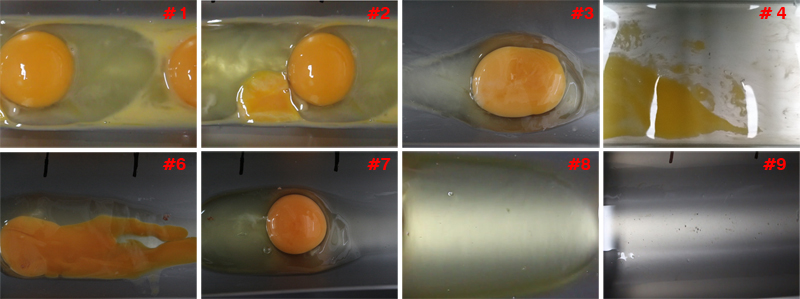
\includegraphics[width=0.8\paperwidth]{8of9}
\caption{Cracked egg product cases. Source: own materials }
\end{figure}
Source: own materials 

Also, a problem is constituted by chalaza – a usually white element that is attached to egg yolk for in-egg suspension.
Despite the fact, that client decided that chalaza position and amount are irrelevant to him, its appearance may increase difficulty of the recognition problem if identified as parts of damaged egg yolk.

 
\begin{figure}[H]
\centering
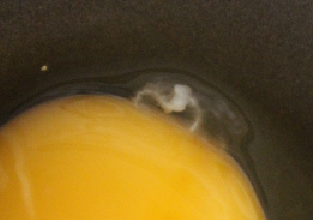
\includegraphics[width=0.4\paperwidth]{chalaza}
\caption{Chalaza attached to egg. Source: own materials}
\end{figure}


\subsection{Techniques of automatic egg quality assessment}

Different techniques for automatic, non-destructive egg quality grading have been investigated.
Among them, the following are worth mentioning:
- Intelligent systems based on visible-infrared transmittance spectroscopy\cite{agri}
- Fourier frequency analysis of a vibration-based response on impact force\cite{svm} 
- Ultrasonic, magnetic resonance, electric resistance, electric nose\cite{nondestr}  
All methods listed above require very specific equipment, are prone to overfitting and take in to account assumption that does not has to be satisfied for problem considered in this thesis: the egg shell should not be damaged.

Since in this very special case, eggs are already broken, simplified and different methods can be considered.
Initially, two ideas were researched by author of this thesis:
- Proximity sensor utilization
- Using laser / narrow light beam 
Both methods would identify the intact yolk basing on its height and wouldn’t require much processing (an Arduino Uno or other ATMega based circuits might be sufficient).

Nevertheless, both of them had to be rejected, since intact yolks presence in the tested batch is not sufficient for batch accepting – absence of egg yolk parts is also required (see subchapter 2.1).

Finally, using images of the batch obtained from camera and processing it was chosen as a most promising option for further research.

\subsection{Detecting batch state with camera image}

When it comes to assessment of camera image, 4 approaches are widely considered:
\begin{enumerate}
\item Very easy scanning with photo sensors or very low resolution cameras
\item Computer graphics preprocessing and segmentation accompanied with assessment of a parameter (number of pixels, number of feature points, percentage of one region that fills another bigger region and similar)
\item Machine learning approach
\item Neural networks which are used as a special case of either machine learning process or a part of it 
\end{enumerate}
First case was considered, since it could be implemented on Arduino Uno, other ATMega based platform or real-time systems working on PLC controllers such as LOGO! 7, which are often used in factories due to their reliability (apart from Stuxnet-class worms, that has been firstly observed in 2010, no other security threads are believed to exist).
Unfortunately, the problem is more complex than simply deciding whether the product is present or not; or whether the product is yellow or not, thus more advanced processing is required.

Second case will be expanded in the next subchapter and has been chosen as main method that will be implemented and tested in this thesis.

Last two approaches will be tested if the 2nd approach will provide to be insufficient.
It is worth mentioning, that for (3) Support Vector Machines was considered, since it classifies data to exactly two classes (i.e. proper and improper egg mass).

Also, Haar Features Cascade was tested, but data amount obtained for testing was insufficient, and the methods popular implementations are focused on locating the particular object on image rather than on comparing two pattern cases.
(4) Case was considered and the author build a multilayered perceptron network working with MNIST database in order to better understand the method.
The method application will be researched further on beyond the scope of this work.





\subsection{Chosen method structure}

Firstly the preprocessing will be done to eliminate unimportant data (reduce the dimensionality), reduce noises and extract interesting image areas.

Secondly the image will be segmented to extract egg yolk (whole and damaged).

Thirdly two options will be tested:
- The undamaged egg yolks will be detected and deleted from the image. Than the amount of remaining yolk parts will be counted. If it will exceed the threshold value, the signal for removing the product batch will be sent.
- The extracted egg yolk will be graded in terms of shape similarity to a single, intact yolk

The best obtained combination of preprocessing, segmentation and grading parameters will be used in a final algorithm that will be implemented in Raspberry Pi 2 device with camera module, and than tested in the Rz-1 processing plant.
\section{Batch state detection system}
\subsection{System design}
lorem ipsum
\subsection{Detection Algorithm}
lorem ipsum
\begin{figure}[H]
\centering
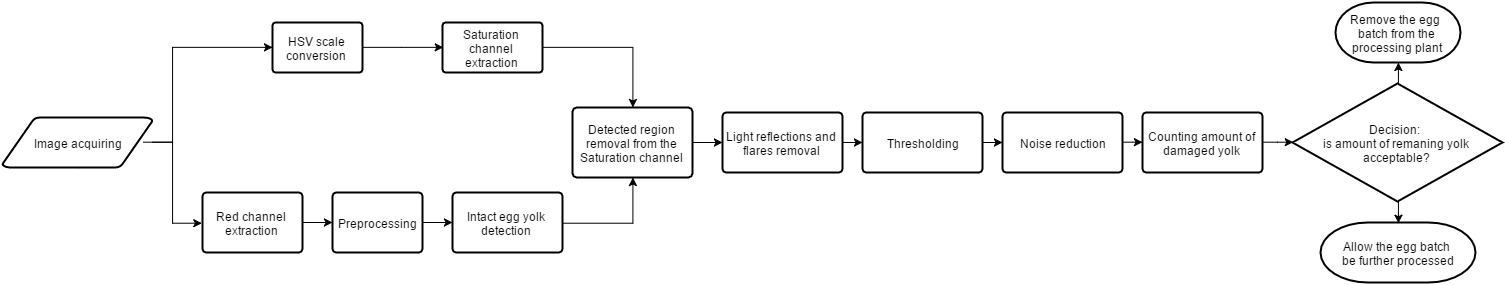
\includegraphics[width=0.8\paperwidth]{algorithm}
\caption{Detection Algorithm}
\end{figure}
lorem ipsum
\section{Egg yolk detection}
\subsection{Methods overview}
An egg yolk, when intact and fresh can be approximated with sphere which projects as circle-like shape on 2D image.
Methods presented below enable to filter out the unnecessary noise, simplify the image and detect the yolk shape.
While not all of them were used in the final detection algorithm, they were giving promising results on the early stage prototypes.

Following methods treat images as 1, 8, or 24-bit encoded matrices, thus both terms are used synonymously. 
x and y denote pixel position.

\subsection{Circle Hough Transform (CHT)}
Circle Hough Transform is an algorithm used for retrieving 3 parameters defining a circle-like shape on images\cite{hgtcv} : 
- (xc, yc) - position of shapes center
- r - its radius

To understand the way CHT works, simplified case is considered:
The image is 1-bit encoded; the radius r and position (xp,yp) of a point lying on the searched circle are known.
Potential circles space is created by treating points on a circle of radius r centered in (xp,yp) as centers for potential circles.
For every potential circle, number of intersecting points is counted.
The potential circle with largest number of intersections is chosen as the best fitting one.

 
\begin{figure}[H]
\centering
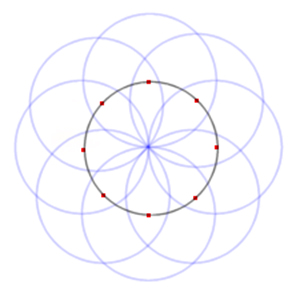
\includegraphics[width=0.4\paperwidth]{space}
\caption{Potential circles space\cite{craters}}
\end{figure}

In the full cases, such procedure is repeated for every image point, and the intersections numbers are stored in accumulation matrix.\cite{hgt}
To reduce computation time and false detection rate, minimum distance between image centers is given as a parameter min-dist.
Threshold value param-2 is defined as minimum number of intersections to treat circle candidate as detected circle.
 
\begin{figure}[H]
\centering
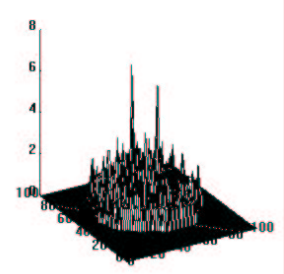
\includegraphics[width=0.4\paperwidth]{accu}
\caption{Accumulation matrix with two good circle candidates\cite{hgt}}
\end{figure}

If r is unknown, min-radius and max-radius parameters are defined, and the algorithm repeats the procedure for all possible integer r in range of above parameters.
OpenCV utilizes Canny edge detector for finding the potential intersection points, thus operates not only on 1-bit images, but also in 8-bit grayscale and 24-bit bgr images and provides smaller number of false positives.\cite{mastercv}
param-1 is introduced as higher threshold for Canny edge detector, while the lower threshold is set to 0.5 * param-1\cite{fd} .


\subsection{Erosion and Dilatation}
Erosion and dilatation are two morphological filters that enable to filter out unnecessary noise from the image.
Combined, they leave the core information (biggest blobs) intact or amplified, while small elements are deleted.
It is easily applied to binary images:
A ROI (region of interest, a rectangular part of image) moves through image pixel by pixel and is compared to previously defined kernel (binary matrix, usually symmetric with respect to both diagonals).

 
\begin{figure}[H]
\centering
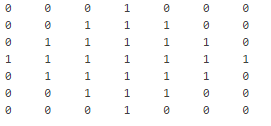
\includegraphics[width=0.4\paperwidth]{diam}
\caption{A diamond-shaped kernel\cite{morph}}
\end{figure}

The consecutive pixels of on ROI that matches kernel elements with value 0 remain intact.
Pixels of ROI that matches kernel 1-valued elements changes to:
1-ns if at least one of them is 1 for Dilatation
0-s if at least one of them is 0 for Erosion.

Erosion gives the effect of ‘shrinking’ the objects (and if they are small enough, they are deleted).
Dilatation makes the objects bigger.

 
\begin{figure}[H]
\centering

\includegraphics[width=0.4\paperwidth]{lett}
\caption{Orignal image, eroded image, dilated image.\cite{erdil}}
\end{figure}


When these methods are used multiple times, and convoluted, they filter out the noise.
Perimeter Determination and Skeletonization are widely used contour detection functions which utilize erosion and dilatation\cite{erdil}.


\subsection{Gaussian blur}

Gaussian blur is obtained by convoluting pixel with gauss function values. 

It reduces noise, detail and filters out the high frequencies what makes it a low pass filter.\cite{cv}

Gaussian blur drastically reduces number of false-positive Hough circles detections. It nevertheless should be coupled with sharpening to reduce false-negative cases.\cite{cnoisy} 


\begin{figure}[H]
\centering
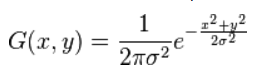
\includegraphics[width=0.4\paperwidth]{gauss}
\caption{Gauss function in two dimension\cite{featproc}}
\end{figure}


sigma, ksize.width, ksize.height  parameters are introducted. 
Ksize stands for size of precomputed kernel, that is convoluted with ROIs on the image.

The term ‘convolution’ might be misleading and for the scope of image processing tasks is defined as picewise multipling two matrices and than summing the obtained values:

 
\begin{figure}[H]
\centering
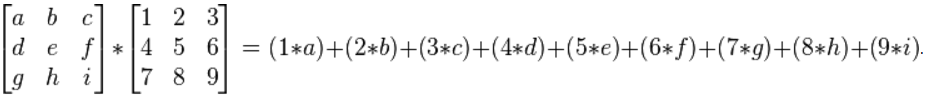
\includegraphics[width=0.8\paperwidth]{conv}
\caption{Convolution of 3x3 matrices\cite{gimp}}
\end{figure}

 
\begin{figure}[H]
\centering
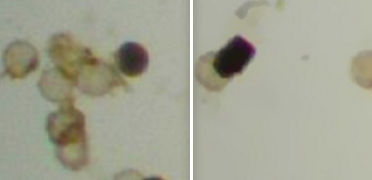
\includegraphics[width=0.4\paperwidth]{micro}
\caption{Microscope image before and after applying gaussian filter\cite{cnoisy}}
\end{figure}

  


\subsection{Channeling and HSV conversion}
lorem ipsum
\subsection{Finding optimal parameter values}
lorem ipsum
\subsection{Overfitting}
lorem ipsum
\section{Contaminated product recognition}
\subsection{General idea}
lorem ipsum
\subsection{Thresholding}

Thresholding is a simple case of image segmentation.
It can be used to convert one channel (in most cases grayscale) image to binary image.
The basic binary thresholding mode sets every pixel of destination matrix to
	0 if the source matrix value is smaller than threshold (integer parameter)
	1 if the source matrix value is bigger than threshold.
The truncate version sets every pixel of destination matrix to
	threshold if the source matrix value is smaller than threshold, or
	leaves it unaltered otherwise.
Various modes and modifications are used depending on coding schema and colors distribution.
  
\begin{figure}[H]
\centering
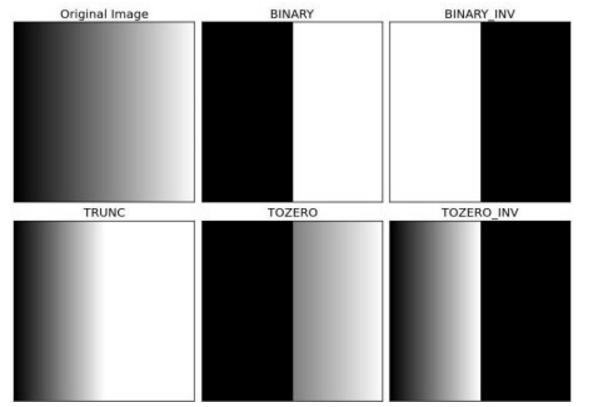
\includegraphics[width=0.4\paperwidth]{thr}
\caption{Different Thresholding modes generated with Metaplotlib}
\end{figure}



Finding optimal threshold value finding is a time consuming process and it often gives satisfactory results only for small set of images.
Therefore Otsu Binarization algorithm for automatically selecting threshold is used.

Moreover using one threshold value for whole image may not work properly if the lighting conditions differ in different image areas.\cite{thre}
Adaptive Thresholding utilize different threshold values for different ROIs. 
Two modes are often used: Adaptive Mean and Adaptive Gaussian.
First compute threshold value as mean of neighborhood values.
Second uses weighted sum neighborhood values.
 
\begin{figure}[H]
\centering
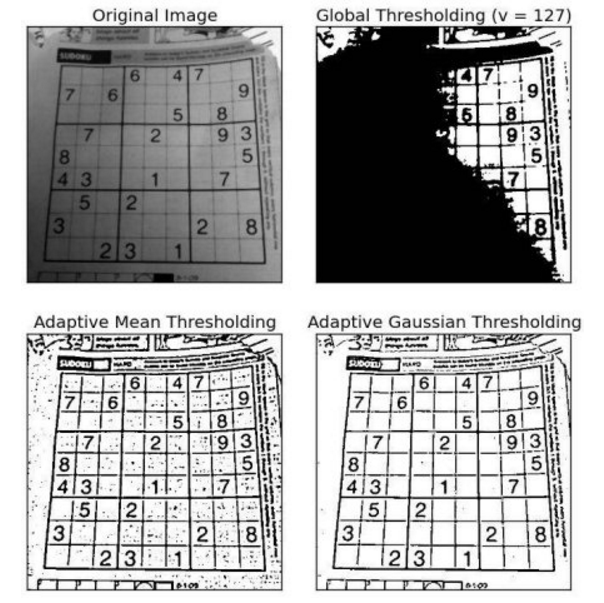
\includegraphics[width=0.4\paperwidth]{thremeth}
\caption{Threshold computing methods12\cite{thre}}
\end{figure}
 
\begin{figure}[H]
\centering
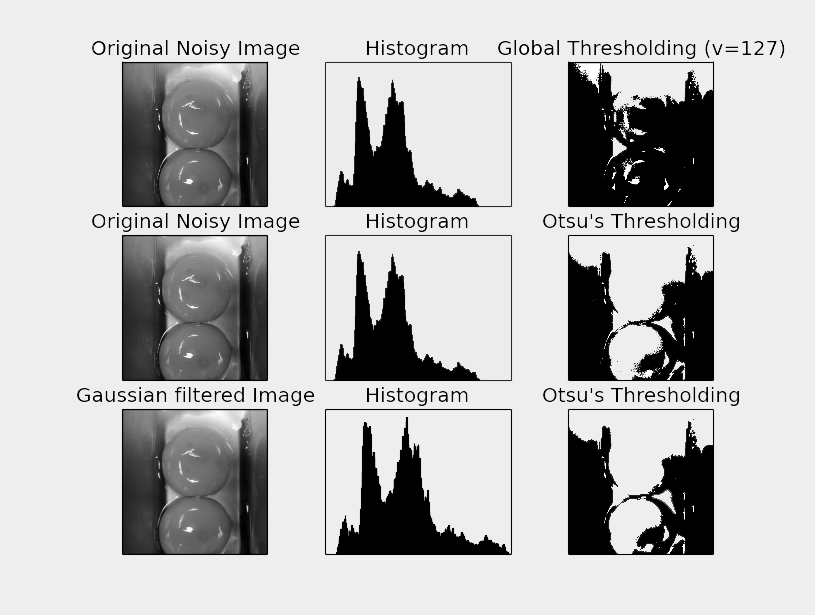
\includegraphics[width=0.4\paperwidth]{diffthr}
\caption{Different thresholding applied
Fig. generated with Metaplotlib}
\end{figure}


For more general cases (i.e. multichannel images, assigning more colors) clustering method known as k-means is widely used.\cite{lesscv}
 
\begin{figure}[H]
\centering
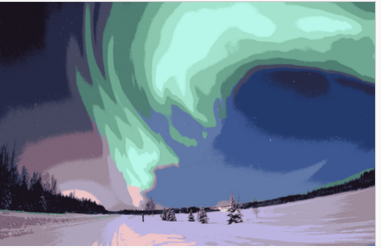
\includegraphics[width=0.4\paperwidth]{kmeans}
\caption{K-means clustering method for k = 16\cite{segm}}
\end{figure}

\section{Choosing detection system parameters}
\subsection{Brute force testing}
lorem ipsum
\section{Phisical system implementation}
\subsection{Raspberry Pi}
lorem ipsum
\section{Conclusions}
\subsection{Beyond the scope}
lorem ipsum


All the Web. sources have been checked for availability in November 2015.
Web links are not included if articles are to be immediately found with search engines, which is consistent to MLN referencing convention.
For modified web documents, date of last modification is shown.


\begin{thebibliography}{9}
 
\bibitem{eggprop} 
Berry D.
\textit{Egg product functional properties} 
American Egg Board Web. 2013

\bibitem{agri} 
Mehdizadeha S., Minaeib S., Hancockc N. H. ,Torshizid M.
\textit{Information Processing in Agriculture}, Volume 1, Issue 2 
Print. 2014

\bibitem{svm} 
Deng X., Wang Q., Chen H., Xie H.
\textit{Eggshell crack detection using a wavelet-based support vector machine} Comput Electron Agric, Print. 2010

\bibitem{nondestr} 
Ketelaerea B.,Bamelisa F., Kempsa1 B., Decuyperea1 E., Baerdemaekera J.
\textit{Non-destructive measurements of the egg quality} World's Poultry Science Journal, Volume 60 / Issue 03,  Cambridge University Press, Print. 2004
 
\bibitem{hgtcv} 
Opencv Dev Team
\textit{Hough Circle Transform} OpenCV 2.4.12.0 Documentation, Web. 2014

\bibitem{craters} 
Milbourne A.
\textit{Computers Counting Craters} Birkbeck College, Web. 2012

\bibitem{hgt} 
Rhody, Harvey
\textit{Hough Circle Transform} Chester F. Carlson Center for Imaging Science Rochester Institute of Technology, Web. 2005

\bibitem{mastercv} 
Kapur S., Thakkar N.
\textit{Mastering OpenCV Android Application Programming} Pack Publishing, Print. 2015

\bibitem{fd} 
Opencv Dev Team
\textit{Feature Detection} OpenCV 2.4.12.0 Documentation, Web. 2014

\bibitem{morph} 
Opencv Dev Team
\textit{Morphology Fundamentals: Dilation and Erosion} MathWorks Documentation, The MathWorks, Inc. Web. 2014

\bibitem{erdil} 
Opencv Dev Team
\textit{Eroding and Dilating} OpenCV 2.4.12.0 Documentation, Opencv Dev Team, Web. 2014

\bibitem{cv} 
Shapiro L. G., Stockman G. C
\textit{Computer Vision} Prentice Hall, Print. 2001

\bibitem{cnoisy} 
Khvedchenya E.
\textit{How to detect circles in noisy images} Computer Vision Talks, Web. 2014

\bibitem{featproc} 
Nixon M. S., Aguado A. S.
\textit{Feature Extraction and Image Processing} Academic Press, Print. 2008

\bibitem{gimp} 
Lecarme  O., Delvare K.
\textit{The Book of GIMP: A Complete Guide to Nearly Everything} No Starch Press, Print. 2013

\bibitem{thre} 
Opencv Dev Team
\textit{Image Thresholding.} OpenCV 2.4.12.0 Documentation, Web. 2014

\bibitem{lesscv} 
Barghout L., Sheynin J.
\textit{Real-world scene perception and perceptual organization: Lessons from Computer Vision.} Journal of Vision, Print. 2013

\bibitem{segm} 
Barghout L., Sheynin J.
\textit{Image segmentation} Wikipedia, Wikimedia Foundation Inc, Web. 2015

\end{thebibliography}


\end{document}